\let\negmedspace\undefined
\let\negthickspace\undefined
\documentclass[journal]{IEEEtran}
\usepackage[a5paper, margin=10mm, onecolumn]{geometry}
%\usepackage{lmodern} % Ensure lmodern is loaded for pdflatex
\usepackage{tfrupee} % Include tfrupee package

\setlength{\headheight}{1cm} % Set the height of the header box
\setlength{\headsep}{0mm}     % Set the distance between the header box and the top of the text
\usepackage{gvv-book}
\usepackage{gvv}
\usepackage{cite}
\usepackage{amsmath,amssymb,amsfonts,amsthm}
\usepackage{algorithmic}
\usepackage{graphicx}
\usepackage{textcomp}
\usepackage{xcolor}
\usepackage{txfonts}
\usepackage{listings}
\usepackage{enumitem}
\usepackage{mathtools}
\usepackage{gensymb}
\usepackage{comment}
\usepackage[breaklinks=true]{hyperref}
\usepackage{tkz-euclide} 
\usepackage{listings}
% \usepackage{gvv}                                        
\def\inputGnumericTable{}                                 
\usepackage[latin1]{inputenc}                                
\usepackage{color}                                            
\usepackage{array}                                            
\usepackage{longtable}                                       
\usepackage{calc}                                             
\usepackage{multirow}                                         
\usepackage{hhline}                                           
\usepackage{ifthen}                                           
\usepackage{lscape}
\usepackage{circuitikz}

\renewcommand{\thefigure}{\theenumi}
\renewcommand{\thetable}{\theenumi}
\setlength{\intextsep}{10pt} % Space between text and floats


\numberwithin{equation}{enumi}
\numberwithin{figure}{enumi}
\renewcommand{\thetable}{\theenumi}




% Marks the beginning of the document
\begin{document}
\bibliographystyle{IEEEtran}
\vspace{3cm}

\title{MA\\2024}
\author{EE24BTECH11063 - Y.Harsha Vardhan Reddy}
\maketitle

\bigskip

\renewcommand{\thefigure}{\theenumi}
\renewcommand{\thetable}{\theenumi}

\section*{Q.1 to Q.5 carry ONE mark each}
\begin{enumerate}
\item
If '$\rightarrow$' denotes increasing order of intensity, then the meaning of the words \\
$[ \text{drizzle} \rightarrow \text{rain} \rightarrow \text{downpour} ]$ is analogous to $[ \underline{\hspace{2cm}} \rightarrow \text{quarrel} \rightarrow \text{feud} ]$. \\
Which one of the given options is appropriate to fill the blank?




\begin{enumerate}
\begin{multicols}{4}
\item bicker
\item bog 
\item dither 
\item dodge 
\end{multicols}
\end{enumerate}

\bigskip

\item Statements: 
\begin{enumerate}[label=\arabic*.]
    \item All heroes are winners.
    \item All winners are lucky people.
\end{enumerate}

Inferences:
\begin{enumerate}[label=\Roman*.]
    \item All lucky people are heroes.
    \item Some lucky people are heroes.
    \item Some winners are heroes.
\end{enumerate}

Which of the above inferences can be logically deduced from statements 1 and 2?



\begin{enumerate}
    \begin{multicols}{2}
        \item  Only I and II
        \columnbreak
        \item  Only II and III
        \end{multicols}
        \begin{multicols}{2}
        \item  Only I and III
        \item  Only III
    \end{multicols}
\end{enumerate}
\bigskip

\item A student was supposed to \textbf{multiply} a positive real number $ p $ with another positive real number $ q $. Instead, the student \textbf{divided} $ p $ by $ q $. If the percentage error in the student's answer is 80\%, the value of $ q $ is 



\begin{enumerate}
    \begin{multicols}{4}
        \item  $ 5 $
        \item  $ \sqrt{2} $
        \item  $ 2 $
        \item  $ \sqrt{5} $
    \end{multicols}
\end{enumerate}
\bigskip

\item If the sum of the first 20 consecutive positive odd numbers is divided by $ 20^2 $, the result is 



\begin{enumerate}
    \begin{multicols}{4}
        \item  $ 1 $
        \item  $ 20 $
        \item  $ 2 $

\item
        \item  $ \frac{1}{2} $
    \end{multicols}
\end{enumerate}
\bigskip

\item If the sum of the first 20 consecutive positive odd numbers is divided by $ 20^2 $, the result is 



\begin{enumerate}
    \begin{multicols}{4}
        \item  $ 1 $
        \item  $ 20 $
        \item  $ 2 $
        \item  $ \frac{1}{2} $
    \end{multicols}
\end{enumerate}
\bigskip

\section*{Q.6 to Q.10 carry TWO marks each}

\item In the given text, the blanks are numbered (i)-(iv). Select the best match for all the blanks.
Yoko Roi stands (i) \underline{\hspace{1cm}} as an author for standing (ii) \underline{\hspace{1cm}} as an honorary fellow, after she stood (iii) \underline{\hspace{1cm}} her writings that stand (iv) \underline{\hspace{1cm}} the freedom of speech.



\begin{enumerate}
    \begin{multicols}{2}
        \item (i) out (ii) down (iii) in (iv) for
        \columnbreak
        \item  (i) down (ii) out (iii) by (iv) in
        \end{multicols}
        \begin{multicols}{2}
        \item  (i) down (ii) out (iii) for (iv) in
        \item  (i) out (ii) down (iii) by (iv) for
        
    \end{multicols}
\end{enumerate}
\bigskip

\item Seven identical cylindrical chalk-sticks are fitted tightly in a cylindrical container. The figure below$\ref{fig:1}$ shows the arrangement of the chalk-sticks inside the cylinder.


The length of the container is equal to the length of the chalk-sticks. The ratio of the occupied space to the empty space of the container is 
\begin{figure}[H]
    
			\centering
			\begin{tikzpicture}
\draw (0,0) node[left] {$P$} -- (4,0) node[right] {$Q$} -- (4,2) node[above] {$R$} -- cycle;
\draw (3,0) node[below] {$S$} -- (2,1) node[above] {$U$} -- (4,1) node[right] {$T$} -- cycle;
\draw (2,1) -- (3,0);
\end{tikzpicture}

			\caption{}
			\label{fig:1}
		\end{figure}

\begin{enumerate}
    \begin{multicols}{4}
        \item  $ \frac{5}{2} $
        \item $ \frac{7}{2} $
        \item  $ \frac{9}{2} $
        \item  $ 3 $
    \end{multicols}
\end{enumerate}
\bigskip

\item The plot below$\ref{fig:2}$ shows the relationship between the mortality risk of cardiovascular disease and the number of steps a person walks per day. Based on the data, which one of the following options is true?
\begin{figure}[H]
    \centering
    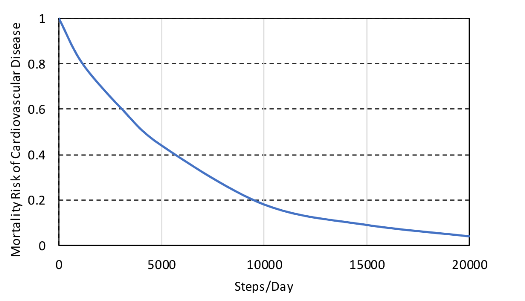
\includegraphics[width=\linewidth]{figs/2.png}
    \caption{Steps/Day}
    \label{fig:2}
    \end{figure}
\begin{enumerate}
        \item  The risk reduction on increasing the steps/day from 0 to 10000 is less than the risk reduction on increasing the steps/day from 10000 to 20000.
        \item  The risk reduction on increasing the steps/day from 0 to 5000 is less than the risk reduction on increasing the steps/day from 15000 to 20000.
        \item  For any 5000 increment in steps/day the largest risk reduction occurs on going from 0 to 5000.
        \item  For any 5000 increment in steps/day the largest risk reduction occurs on going from 15000 to 20000.
    

\end{enumerate}

\bigskip
\item
Five cubes of identical size and another smaller cube are assembled as shown in Figure A$\ref{fig:3}$. If viewed from direction $ X $, the planar image of the assembly appears as Figure B.

\begin{figure}[H]
    
			\centering
			\begin{circuitikz}
            \tikzstyle{every node}=[font=\normalsize]

            % First XOR Gate
            \draw (10,19.25) to[short] (10.25,19.25);
            \draw (10,18.75) to[short] (10.25,18.75);
            \draw (10.25,19.25) node[ieeestd xor port, anchor=in 1, scale=0.89](xor1){} 
                  (xor1.out) to[short] (12,19);
            
            % Second XOR Gate
            \draw (10,17.25) to[short] (10.25,17.25);
            \draw (10,16.75) to[short] (10.25,16.75);
            \draw (10.25,17.25) node[ieeestd xor port, anchor=in 1, scale=0.89](xor2){} 
                  (xor2.out) to[short] (12,17);
            
            % Third XOR Gate
            \draw (14.75,18.25) to[short] (15,18.25);
            \draw (14.75,17.75) to[short] (15,17.75);
            \draw (15,18.25) node[ieeestd xor port, anchor=in 1, scale=0.89](xor3){} 
                  (xor3.out) to[short] (16.75,18);
            
            % Connections for inputs
            \draw (8.25,19.25) to[short] (10.25,19.25);
            \draw (8.25,18.75) to[short] (10.25,18.75);
            \draw (8.25,17.25) to[short] (10.25,17.25);
            \draw (8.25,16.75) to[short] (10.25,16.75);
            
            % Inter-gate connections
            \draw (13.25,18.25) to[short] (15.25,18.25);
            \draw (13.25,17.75) to[short] (15.25,17.75);
            \draw (16.75,18) to[short] (18.75,18);
            \draw (11.75,19) to[short] (13.25,19);
            \draw (11.75,17) to[short] (13.25,17);
            \draw (13.25,19) to[short] (13.25,18.25);
            \draw (13.25,17) to[short] (13.25,17.75);
            
            % Labels
            \node [font=\LARGE] at (7.75,19.5) {A};
            \node [font=\LARGE] at (7.75,18.75) {B};
            \node [font=\LARGE] at (7.75,17.25) {C};
            \node [font=\LARGE] at (7.75,16.5) {D};
            \node [font=\LARGE] at (19.25,18) {Y};
            \node [font=\normalsize] at (11,17) {XOR};
            \node [font=\normalsize] at (15.75,18) {XOR};
            \node [font=\normalsize] at (11,19) {XOR};
        \end{circuitikz}

			\caption{}
			\label{fig:3}
		\end{figure}

If viewed from direction $ Y $, the planar image of the assembly (Figure A) will appear as:
\begin{enumerate}

    \item[]

    \begin{figure}[H]
        \centering

        \begin{minipage}{0.45\linewidth}
            \centering
            \begin{circuitikz}
\tikzstyle{every node}=[font=\LARGE]
\draw (9,7.25) to[short] (9,7.25);
\draw (5.75,7.75) to[short] (7.75,7.75);
\draw (7.75,7.75) to[short] (7.75,9.75);
\draw (5.75,8.75) to[short] (7.75,8.75);
\draw (6.75,7.75) to[short] (6.75,9.75);
\draw (6.75,9.75) to[short] (7.75,9.75);
\draw (5.75,7.75) to[short] (5.75,8.75);
\draw (7.25,9.25) to[short] (7.25,8.75);
\draw (7.25,9.25) to[short] (7.75,9.25);
\end{circuitikz}

            \caption*{(a)}
        \end{minipage}%
        \hfill
        \begin{minipage}{0.45\linewidth}
            \centering
            \begin{circuitikz}
\tikzstyle{every node}=[font=\LARGE]
\draw (9,7.25) to[short] (9,7.25);
\draw (5.75,7.75) to[short] (7.75,7.75);
\draw (7.75,7.75) to[short] (7.75,9.75);
\draw (5.75,8.75) to[short] (7.75,8.75);
\draw (6.75,7.75) to[short] (6.75,9.75);
\draw (6.75,9.75) to[short] (7.75,9.75);
\draw (5.75,7.75) to[short] (5.75,8.75);
\draw (7.25,9.25) to[short] (7.25,8.75);
\draw (7.25,9.25) to[short] (7.25,9.75);
\end{circuitikz}

            \caption*{(b)}
        \end{minipage}

    \end{figure}

    \item[]

    \begin{figure}[H]
        \centering

        \begin{minipage}{0.45\linewidth}
            \centering
            \begin{circuitikz}
\tikzstyle{every node}=[font=\LARGE]
\draw (9,7.25) to[short] (9,7.25);
\draw (5.75,7.75) to[short] (7.75,7.75);
\draw (7.75,7.75) to[short] (7.75,9.75);
\draw (5.75,8.75) to[short] (7.75,8.75);
\draw (6.75,7.75) to[short] (6.75,9.75);
\draw (6.75,9.75) to[short] (7.75,9.75);
\draw (5.75,7.75) to[short] (5.75,8.75);
\draw (7.25,9.25) to[short] (7.25,8.75);
\draw (7.25,9.25) to[short] (6.75,9.25);
\end{circuitikz}

            \caption*{(c)}
        \end{minipage}%
        \hfill
        \begin{minipage}{0.45\linewidth}
            \centering
            \begin{circuitikz}
\tikzstyle{every node}=[font=\LARGE]
\draw (9,7.25) to[short] (9,7.25);
\draw (5.75,7.75) to[short] (7.75,7.75);
\draw (7.75,7.75) to[short] (7.75,9.75);
\draw (5.75,8.75) to[short] (7.75,8.75);
\draw (6.75,7.75) to[short] (6.75,9.75);
\draw (6.75,9.75) to[short] (7.75,9.75);
\draw (5.75,7.75) to[short] (5.75,8.75);
\draw (6.25,9.25) to[short] (6.25,8.75);
\draw (6.75,9.25) to[short] (6.25,9.25);
\end{circuitikz}

            \caption*{(d)}
        \end{minipage}

    \end{figure}
    
\end{enumerate}

\bigskip


\item

Visualize a cube that is held with one of the four body diagonals aligned to the vertical axis. Rotate the cube about this axis such that its view remains unchanged. The magnitude of the minimum angle of rotation is 


\begin{enumerate}
    \begin{multicols}{4}
        \item  $ 120^\circ $
        \item $ 60^\circ $
        \item  $ 90^\circ $
        \item  $ 180^\circ $
    \end{multicols}
\end{enumerate}

\bigskip

\section*{MCQ}
\item 

Consider the following condition on a function $ f : \mathbb{C} \to \mathbb{C} $

$
|f(z)| = 1 \quad \text{for all } z \in \mathbb{C} \text{ such that } \text{Im}(z) = 0. \quad (P)
$

Which one of the following is correct?


\begin{enumerate}
        \item There is a non-constant analytic polynomial $ f $ satisfying (\textbf{P})
        \item  Every entire function $ f $ satisfying (\textbf{P}) is a constant function
        \item Every entire function $ f $ satisfying (\textbf{P}) has no zeroes in $ \mathbb{C} $
        \item  There is an entire function $ f $ satisfying (\textbf{P}) with infinitely many zeroes in $ \mathbb{C} $
\end{enumerate}


\bigskip

\item 

Let $ C $ be the ellipse $ \{ z \in \mathbb{C} : |z - 2| + |z + 2| = 8 \} $ traversed counter-clockwise. The value of the contour integral 

\begin{align*}
\oint_C \frac{z^2 \, dz}{z^2 - 2z + 2}
\end{align*}

is equal to 

\begin{enumerate}
    \begin{multicols}{4}
        \item  $ 0 $
        \item  $ 2\pi i $
        \item  $ 4\pi i $
        \item  $ -\pi i $
    \end{multicols}
\end{enumerate}

\bigskip
\item Let $ X $ be a topological space and $ A \subseteq X $. Given a subset $ S $ of $ X $, let $\text{int}(S)$, $\partial S$, and $\overline{S}$ denote the interior, boundary, and closure, respectively, of the set $ S $. Which one of the following is NOT necessarily true?

\vspace{0.5cm}

\begin{enumerate}
        \item  $ \text{int}(X \setminus A) \subseteq X \setminus \overline{A} $
        \item  $ A \subseteq \overline{A} $
        \item  $ \partial A \subseteq \partial (\text{int}(A)) $
        \item  $ \partial (\overline{A}) \subseteq \partial A $
\end{enumerate}
\end{enumerate}

\end{document}
    
